% -----------------------------*- LaTeX -*------------------------------
\documentclass[UTF8]{report}
% ------------------------------------------------------------------------
% Packages
% ------------------------------------------------------------------------
\usepackage{adjustbox}
\usepackage{algorithm,algorithmicx}
\usepackage[noend]{algpseudocode}
\usepackage{amsmath,amsfonts,amssymb,bm,amsthm} % 数学宏包、数学字体、数学符号、支持 \mathscr{} 字体、支持粗斜体 \bm{}、数学定理
\usepackage{bigstrut,multirow,rotating} % Excel表格自动导入latex
\usepackage{booktabs}
\usepackage{breqn}
\usepackage{caption}
\usepackage{color} % 支持颜色改变
\usepackage{ctex}
\usepackage{enumitem} % 自定义列表环境
\usepackage{esint} % 支持多种积分算子
\usepackage{extarrows} % 任意长度的箭头
\usepackage{fancyhdr}
\usepackage{fontsize}
\usepackage{fontspec}
\usepackage[body={7in, 9in},left=1in,right=1in]{geometry}
\usepackage{graphicx} % 支持 \includegraphics{} 插图
\usepackage{mathrsfs}
\usepackage{mathtools} % 数学宏包的重要补充
\usepackage[framemethod=TikZ]{mdframed}
\usepackage{nicefrac}
\usepackage{scribe}
\usepackage{subfigure} % 插入子图
\usepackage{tikz,xcolor} % 画图、画 Feynman 图
\usepackage{upgreek} % 数学环境的直立希腊字母
\usepackage{colortbl} % 表格颜色
% ------------------------------------------------------------------------
% Macros
% ------------------------------------------------------------------------
%~~~~~~~~~~~~~~~
% Utility latin
%~~~~~~~~~~~~~~~
\newcommand{\ie}{\textit{i.e.}}
\newcommand{\eg}{\textit{e.g.}}
%~~~~~~~~~~~~~~~
% Environment shortcuts
%~~~~~~~~~~~~~~~
\newcommand{\balign}[1]{\ealign{\begin{align}#1\end{align}}}
\newcommand{\baligns}[1]{\ealigns{\begin{align*}#1\end{align*}}}
\newcommand{\bitemize}[1]{\eitemize{\begin{itemize}#1\end{itemize}}}
\newcommand{\benumerate}[1]{\eenumerate{\begin{enumerate}#1\end{enumerate}}}
%~~~~~~~~~~~~~~~
% Text with quads around it
%~~~~~~~~~~~~~~~
\newcommand{\qtext}[1]{\quad\text{#1}\quad}
%~~~~~~~~~~~~~~~
% Shorthand for math formatting
%~~~~~~~~~~~~~~~
\newcommand{\mbb}[1]{\mathbb{#1}}
\newcommand{\mbi}[1]{\boldsymbol{#1}} % Bold and italic (math bold italic)
\newcommand{\mbf}[1]{\mathbf{#1}}
\newcommand{\mc}[1]{\mathcal{#1}}
\newcommand{\mrm}[1]{\mathrm{#1}}
\newcommand{\tbf}[1]{\textbf{#1}}
\newcommand{\tsc}[1]{\textsc{#1}}
% \def\<{{\langle}}
% \def\>{{\rangle}}
\newcommand{\sT}{\sf T}
\newcommand{\grad}{\nabla}
\newcommand{\Proj}{\Pi}
%~~~~~~~~~~~~~~~
% Common sets 定义数集符号
%~~~~~~~~~~~~~~~
\newcommand{\R}{\mathbb{R}}
\newcommand{\Z}{\mathbb{Z}}
\newcommand{\Q}{\mathbb{Q}}
\newcommand{\N}{\mathbb{N}}
\newcommand{\C}{\mathbb{C}}
\newcommand{\reals}{\mathbb{R}} % Real number symbol
\newcommand{\integers}{\mathbb{Z}} % Integer symbol
\newcommand{\rationals}{\mathbb{Q}} % Rational numbers
\newcommand{\naturals}{\mathbb{N}} % Natural numbers
\newcommand{\complex}{\mathbb{C}} % Complex numbers
%~~~~~~~~~~~~~~~
% Common functions
%~~~~~~~~~~~~~~~
\renewcommand{\exp}[1]{\operatorname{exp}\left(#1\right)} % Exponential
\newcommand{\indic}[1]{\mbb{I}\left(#1\right)} % Indicator function
\newcommand{\indicsub}[2]{\mbb{I}_{#2}\left(#1\right)} % Indicator function
\newcommand{\argmax}{\mathop\mathrm{arg\, max}} % Defining math symbols
\newcommand{\argmin}{\mathop\mathrm{arg\, min}}
\renewcommand{\arccos}{\mathop\mathrm{arccos}}
\newcommand{\dom}{\mathop\mathrm{dom}} % Domain
\newcommand{\range}{\mathop\mathrm{range}} % Range
\newcommand{\diag}{\mathop\mathrm{diag}}
\newcommand{\tr}{\mathop\mathrm{tr}}
\newcommand{\abs}{\mathop\mathrm{abs}}
\newcommand{\card}{\mathop\mathrm{card}}
\newcommand{\sign}{\mathop\mathrm{sign}}
\newcommand{\prox}{\mathrm{prox}} % prox
\newcommand{\rank}[1]{\mathrm{rank}(#1)}
\newcommand{\supp}[1]{\mathrm{supp}(#1)}
\newcommand{\norm}[1]{\lVert#1\rVert}
%~~~~~~~~~~~~~~~
% Common probability symbols
%~~~~~~~~~~~~~~~
\newcommand{\family}{\mathcal{P}} % probability family / statistical model
\newcommand{\iid}{\stackrel{\mathrm{iid}}{\sim}}
\newcommand{\ind}{\stackrel{\mathrm{ind}}{\sim}}
\newcommand{\E}{\mathbb{E}} % Expectation symbol
\newcommand{\Earg}[1]{\E\left[#1\right]}
\newcommand{\Esubarg}[2]{\E_{#1}\left[#2\right]}
\renewcommand{\P}{\mathbb{P}} % Probability symbol
\newcommand{\Parg}[1]{\P\left(#1\right)}
\newcommand{\Psubarg}[2]{\P_{#1}\left[#2\right]}
% \newcommand{\Cov}{\mrm{Cov}} % Covariance symbol
% \newcommand{\Covarg}[1]{\Cov\left[#1\right]}
% \newcommand{\Covsubarg}[2]{\Cov_{#1}\left[#2\right]}
% \newcommand{\model}{\mathcal{P}} % probability family / statistical model
%~~~~~~~~~~~~~~~
% Distributions
%~~~~~~~~~~~~~~~
% \newcommand{\Gsn}{\mathcal{N}}
% \newcommand{\Ber}{\textnormal{Ber}}
% \newcommand{\Bin}{\textnormal{Bin}}
% \newcommand{\Unif}{\textnormal{Unif}}
% \newcommand{\Mult}{\textnormal{Mult}}
% \newcommand{\NegMult}{\textnormal{NegMult}}
% \newcommand{\Dir}{\textnormal{Dir}}
% \newcommand{\Bet}{\textnormal{Beta}}
% \newcommand{\Gam}{\textnormal{Gamma}}
% \newcommand{\Poi}{\textnormal{Poi}}
% \newcommand{\HypGeo}{\textnormal{HypGeo}}
% \newcommand{\GEM}{\textnormal{GEM}}
% \newcommand{\BP}{\textnormal{BP}}
% \newcommand{\DP}{\textnormal{DP}}
% \newcommand{\BeP}{\textnormal{BeP}}
% \newcommand{\Exp}{\textnormal{Exp}}
%~~~~~~~~~~~~~~~
% Theorem-like environments
%~~~~~~~~~~~~~~~
% \theoremstyle{definition}
% \newtheorem{definition}{Definition}
% \newtheorem{example}{Example}
% \newtheorem{problem}{Problem}
% \newtheorem{lemma}{Lemma}
%~~~~~~~~~~~~~~~
% 组合数学的模板和作业里用到的一些宏包和自定义命令
%~~~~~~~~~~~~~~~
\renewcommand{\emph}[1]{\begin{kaishu}#1\end{kaishu}}
\newcommand{\falfac}[1]{^{\underline{#1}}}
\newcommand{\binomfrac}[2]{\frac{#1^{\underline{#2}}}{#2!}}
\newcommand{\ceil}[1]{\left\lceil #1 \right\rceil}
\newcommand{\floor}[1]{\left\lfloor #1 \right\rfloor}
\newcommand{\suminfty}[2]{\sum_{#1=#2}^{\infty}}
\newcommand{\suminftyk}[0]{\sum_{k=0}^{\infty}}
\newcommand{\sumint}[3]{\sum_{#1=#2}^{#3}}
\newcommand{\sumintk}[2]{\sum_{k=#1}^{#2}}
\newcommand{\suminti}[2]{\sum_{i=#1}^{#2}}
%~~~~~~~~~~~~~~~
% 定义新命令
%~~~~~~~~~~~~~~~
\newcommand*{\unit}[1]{\mathop{}\!\mathrm{#1}}
\newcommand*{\dif}{\mathop{}\!\mathrm{d}}%微分算子 d
\newcommand*{\pdif}{\mathop{}\!\partial}%偏微分算子
\newcommand*{\cdif}{\mathop{}\!\nabla}%协变导数、nabla 算子
\newcommand*{\laplace}{\mathop{}\!\Delta}%laplace 算子
\newcommand*{\deriv}[2]{\frac{\mathrm{d} #1}{\mathrm{d} {#2}}}
\newcommand*{\derivh}[3]{\frac{\mathrm{d}^{#1} #2}{\mathrm{d} {#3^{#1}}}}
\newcommand*{\pderiv}[2]{\frac{\partial #1}{\partial {#2}}}
\newcommand*{\pderivh}[3]{\frac{\partial^{#1} #2}{\partial {#3^{#1}}}}
\newcommand*{\dderiv}[2]{\dfrac{\mathrm{d} #1}{\mathrm{d} {#2}}}
\newcommand*{\dderivh}[3]{\dfrac{\mathrm{d}^{#1} #2}{\mathrm{d} {#3^{#1}}}}
\newcommand*{\dpderiv}[2]{\dfrac{\partial #1}{\partial {#2}}}
\newcommand*{\dpderivh}[3]{\dfrac{\partial^{#1} #2}{\partial {#3^{#1}}}}
\newcommand{\me}[1]{\mathrm{e}^{#1}}%e 指数
\newcommand{\mi}{\mathrm{i}}%虚数单位
% \newcommand{\mc}{\mathrm{c}}%光速 定义与mathcal冲突
\newcommand{\red}[1]{\textcolor{red}{#1}}
\newcommand{\blue}[1]{\textcolor{blue}{#1}}
% \newcommand{\Rome}[1]{\setcounter{rome}{#1}\Roman{rome}}
%~~~~~~~~~~~~~~~
% 公式环境中箭头符号的简写
%~~~~~~~~~~~~~~~
\newcommand{\ra}{\rightarrow}
\newcommand{\Ra}{\Rightarrow}
\newcommand{\la}{\leftarrow}
\newcommand{\La}{\Leftarrow}
\newcommand{\lra}{\leftrightarrow}
\newcommand{\Lra}{\Leftrightarrow}
\newcommand{\lgla}{\longleftarrow}
\newcommand{\Lgla}{\Longleftarrow}
\newcommand{\lgra}{\longrightarrow}
\newcommand{\Lgra}{\Longrightarrow}
\newcommand{\lglra}{\longleftrightarrow}
\newcommand{\Lglra}{\Longleftrightarrow}
%~~~~~~~~~~~~~~~
% 一些数学的环境设置
%~~~~~~~~~~~~~~~
% \newcounter{counter_exm}\setcounter{counter_exm}{1}
% \newcounter{counter_prb}\setcounter{counter_prb}{1}
% \newcounter{counter_thm}\setcounter{counter_thm}{1}
% \newcounter{counter_lma}\setcounter{counter_lma}{1}
% \newcounter{counter_dft}\setcounter{counter_dft}{1}
% \newcounter{counter_clm}\setcounter{counter_clm}{1}
% \newcounter{counter_cly}\setcounter{counter_cly}{1}
% \newtheorem{theorem}{{\hskip 1.7em \bf 定理}}
% \newtheorem{lemma}[theorem]{\hskip 1.7em 引理}
% \newtheorem{proposition}[theorem]{Proposition}
% \newtheorem{claim}[theorem]{\hskip 1.7em 命题}
% \newtheorem{corollary}[theorem]{\hskip 1.7em 推论}
% \newtheorem{definition}[theorem]{\hskip 1.7em 定义}
\newcommand{\problem}[1]{{\setlength{\parskip}{10pt}\noindent \bf{#1}}}
\newenvironment{solution}{{\noindent\hskip 2em \bf 解 \quad}}{}
\renewenvironment{proof}{{\setlength{\parskip}{7pt}\noindent\hskip 2em \bf 证明 \quad}}{\hfill$\qed$\par}
% \newenvironment{example}{{\noindent\hskip 2em \bf 例 \arabic{counter_exm}\quad}}{\addtocounter{counter_exm}{1}\par}
% \newenvironment{concept}[1]{{\bf #1\quad} \begin{kaishu}} {\end{kaishu}\par}
%~~~~~~~~~~~~~~~
% 本.tex文档中特殊定义命令
%~~~~~~~~~~~~~~~
\newcommand{\cdclass}[2]{[#1]_{\text{#2}}}

% ----------------------------------------------------------------------
% Header information
% ------------------------------------------------------------------------

\begin{document}

\course{B0911006Y-01} 			%optional
\coursetitle{Computer Organization and Design}	%optional
\semester{2023 Spring}		%optional
\lecturer{Ke Zhang}	%optional
\scribe{吉骏雄}		%required
\lecturenumber{14}			%required (must be a number)
\lecturedate{June 25}	%required (omit year)

\maketitle

% ----------------------------------------------------------------------
% Body of the document
% ------------------------------------------------------------------------


\textbf{《计算机组成原理》(唐朔飞版)课后习题8.24~8.28}

\problem{8.24} 现有$A, B, C, D$ $4$个中断源, 其优先级由高向低按$A \to B \to C \to D \to $顺序排列. 若中断服务程序的执行时间为$20 \mathop{}\!\mu \mrm s$, 根据题目图片所示时间轴给出的中断源请求中断的时刻, 画出CPU执行程序的轨迹. 

\begin{solution}
    如图\ref{fig:8_24}所示. 
    \begin{figure}[htbp]
        \centering
        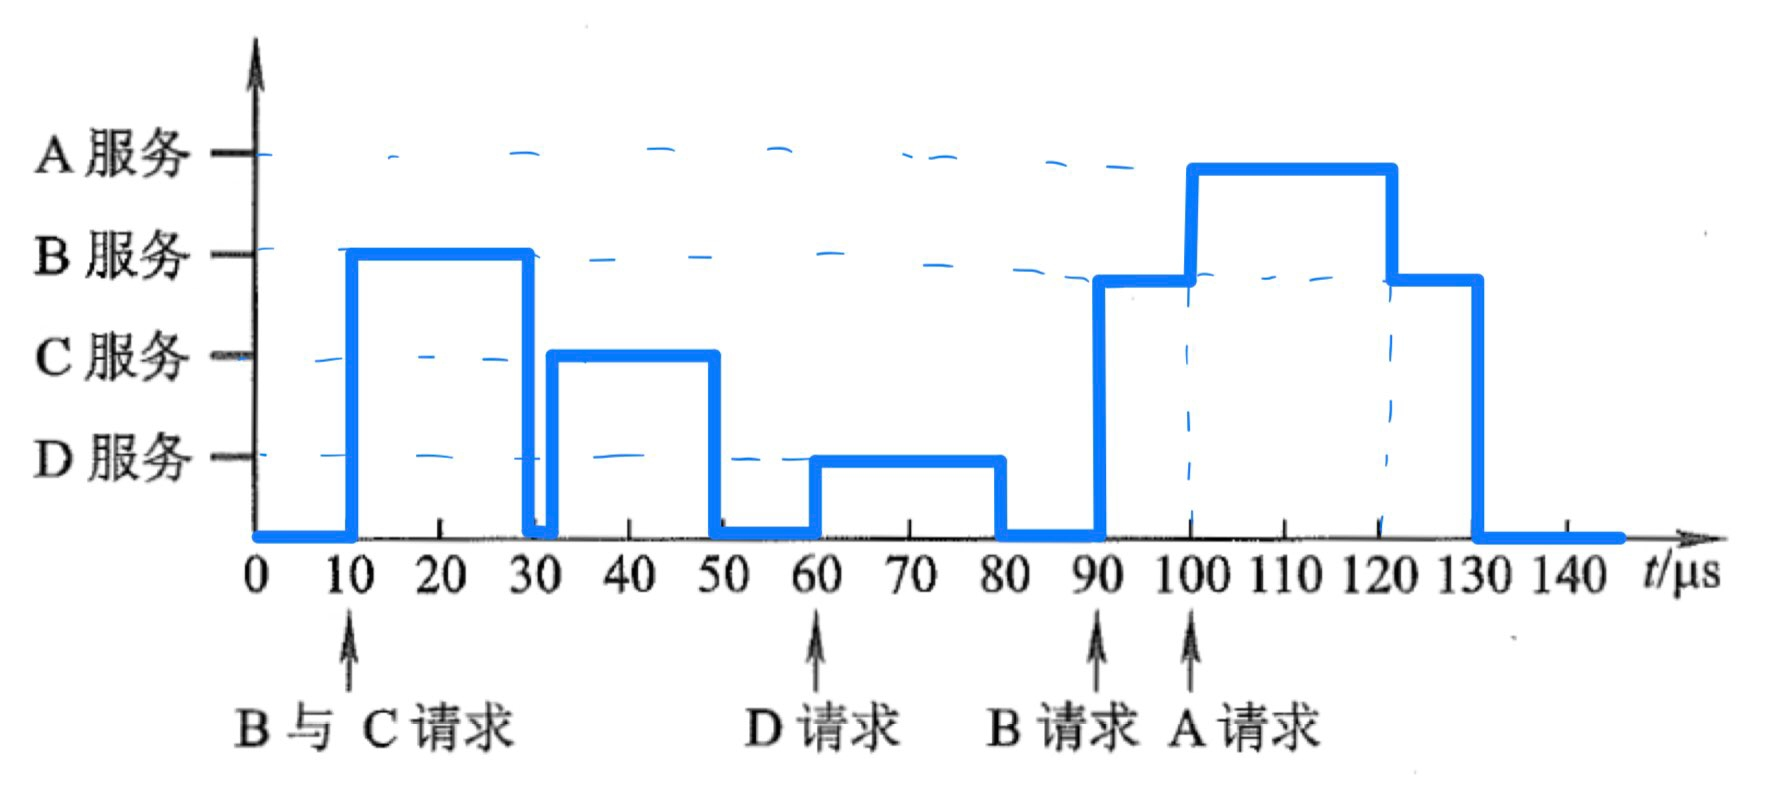
\includegraphics[width=8cm]{fig/8.24.png}
        \caption{题8.24}
        \label{fig:8_24}
    \end{figure}
\end{solution}


\problem{8.25} 设某机有$5$个中断源$L_0,\ L_1,\ L_2,\ L_3,\ L_4$, 按中断响应的优先次序由高向低排序为$L_0 \to L_1 \to L_2 \to L_3 \to L_4$, 现要求中断处理次序改为$L_1 \to L_4 \to L_2 \to L_0 \to L_3$, 根据下面的格式, 写出各中断源的屏蔽字. 

\begin{solution}
    如表\ref{tab:8_25}所示.
\end{solution}

\begin{figure}
    \begin{minipage}[b]{.5\linewidth}
        \centering
        \captionof{table}{题8.25屏蔽字}
        \begin{tabular}{|c|c|c|c|c|c|}
            \hline
            \rowcolor[rgb]{ .894,  .875,  .925}  & \multicolumn{5}{c|}{屏蔽字} \bigstrut\\
            \cline{2-6}  \rowcolor[rgb]{ .894,  .875,  .925} \multirow{-1.5}[4]{*}{中断源}   & 0 & 1 & 2 & 3 & 4 \bigstrut\\
            \hline
            \rowcolor[rgb]{ .773,  .851,  .945} $L_0$ & \cellcolor[rgb]{ .855,  .933,  .953}1 & \cellcolor[rgb]{ .922,  .945,  .871}0 & \cellcolor[rgb]{ .922,  .945,  .871}0 & \cellcolor[rgb]{ .855,  .933,  .953}1 & \cellcolor[rgb]{ .922,  .945,  .871}0 \bigstrut\\
            \hline
            \rowcolor[rgb]{ .773,  .851,  .945} $L_1$ & \cellcolor[rgb]{ .855,  .933,  .953}1 & \cellcolor[rgb]{ .855,  .933,  .953}1 & \cellcolor[rgb]{ .855,  .933,  .953}1 & \cellcolor[rgb]{ .855,  .933,  .953}1 & \cellcolor[rgb]{ .855,  .933,  .953}1 \bigstrut\\
            \hline
            \rowcolor[rgb]{ .773,  .851,  .945} $L_2$ & \cellcolor[rgb]{ .855,  .933,  .953}1 & \cellcolor[rgb]{ .922,  .945,  .871}0 & \cellcolor[rgb]{ .855,  .933,  .953}1 & \cellcolor[rgb]{ .855,  .933,  .953}1 & \cellcolor[rgb]{ .922,  .945,  .871}0 \bigstrut\\
            \hline
            \rowcolor[rgb]{ .773,  .851,  .945} $L_3$ & \cellcolor[rgb]{ .922,  .945,  .871}0 & \cellcolor[rgb]{ .922,  .945,  .871}0 & \cellcolor[rgb]{ .922,  .945,  .871}0 & \cellcolor[rgb]{ .855,  .933,  .953}1 & \cellcolor[rgb]{ .922,  .945,  .871}0 \bigstrut\\
            \hline
            \rowcolor[rgb]{ .773,  .851,  .945} $L_4$ & \cellcolor[rgb]{ .855,  .933,  .953}1 & \cellcolor[rgb]{ .922,  .945,  .871}0 & \cellcolor[rgb]{ .855,  .933,  .953}1 & \cellcolor[rgb]{ .855,  .933,  .953}1 & \cellcolor[rgb]{ .855,  .933,  .953}1 \bigstrut\\
            \hline
        \end{tabular}%
        \label{tab:8_25}%
    \end{minipage}
    \begin{minipage}[b]{.5\linewidth}
        \centering
        \captionof{table}{题8.26屏蔽字}
        \begin{tabular}{|c|c|c|c|}
            \hline
            \rowcolor[rgb]{ .894,  .875,  .925}  & \multicolumn{3}{c|}{屏蔽字} \bigstrut\\
            \cline{2-4}    \rowcolor[rgb]{ .894,  .875,  .925} \multirow{-1.5}[4]{*}{设备}  & A & B & C \bigstrut\\
            \hline
            \rowcolor[rgb]{ .773,  .851,  .945} A & \cellcolor[rgb]{ .855,  .933,  .953}1 & \cellcolor[rgb]{ .855,  .933,  .953}1 & \cellcolor[rgb]{ .855,  .933,  .953}1 \bigstrut\\
            \hline
            \rowcolor[rgb]{ .773,  .851,  .945} B & \cellcolor[rgb]{ .922,  .945,  .871}0 & \cellcolor[rgb]{ .855,  .933,  .953}1 & \cellcolor[rgb]{ .922,  .945,  .871}0 \bigstrut\\
            \hline
            \rowcolor[rgb]{ .773,  .851,  .945} C & \cellcolor[rgb]{ .922,  .945,  .871}0 & \cellcolor[rgb]{ .855,  .933,  .953}1 & \cellcolor[rgb]{ .855,  .933,  .953}1 \bigstrut\\
            \hline
        \end{tabular}%
        \label{tab:8_26}%
    \end{minipage}
\end{figure}

    

\problem{8.26} 设某机配有$A,\ B,\ C$ 3台设备, 其优先级按$A \to B \to C$降序排列, 为改变中断处理次序, 它们的中断屏蔽字设置如下:
% 下面生成一段 LaTeX 代码, 用于生成三线表. 共四行两列, 第一行分别是设备, 屏蔽字两个词. 设备分别是A, B, C; 屏蔽字分别是1 1 1, 0 1 0, 0 1 1
按图示时间轴给出的设备请求中断的时刻,画出CPU执行程序的轨迹。设$A,\ B,\ C$中断服务程序的执行时间均为$20 \mathop{}\!\mu \mrm s$. 


\begin{solution}
    如图\ref{fig:8_26}所示. 
    \begin{figure}[htbp]
        \centering
        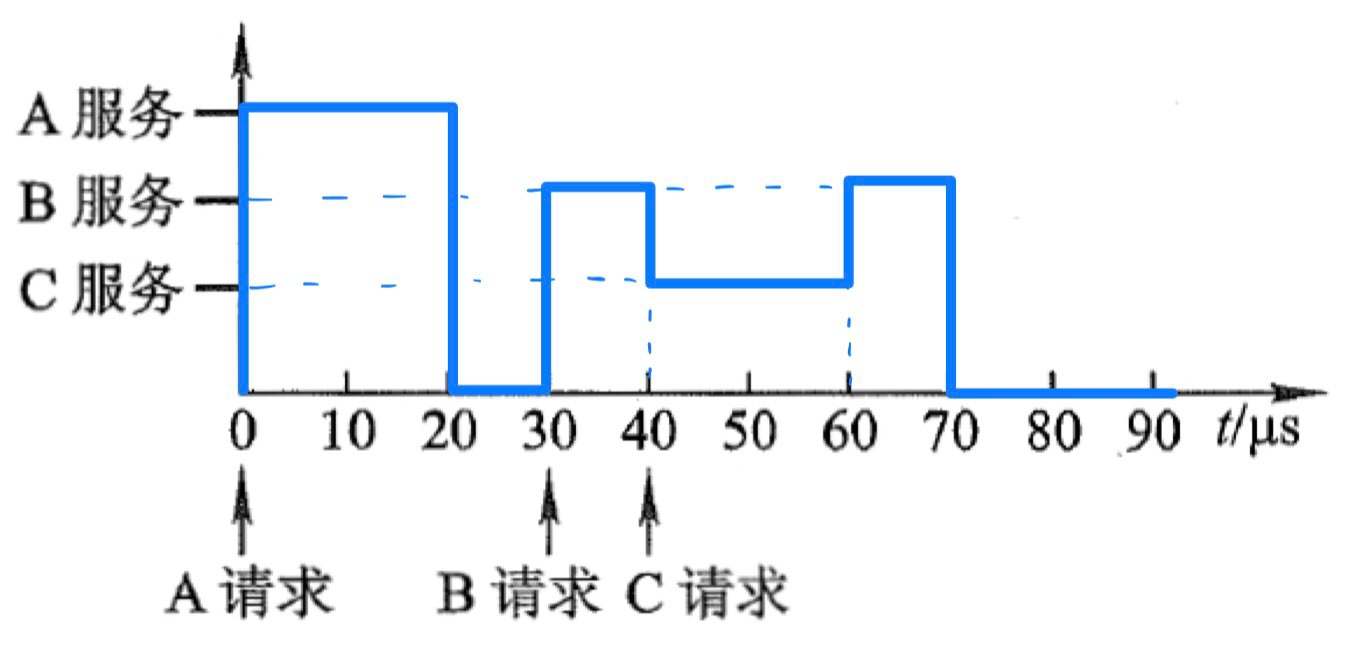
\includegraphics[width=8cm]{fig/8.26.png}
        \caption{题8.26}
        \label{fig:8_26}
    \end{figure}
\end{solution}
    

\problem{8.27} 设某机有$3$个中断源, 其优先级按$1 \to 2 \to 3$降序排列. 假设中断处理时间均为$\tau$, 在下图所示的时间内共发生$5$次中断请求, 图中心表示$1$级中断源发出中断请求信号, 其余类推, 画出CPU执行程序的轨迹.

\begin{solution}
    如图\ref{fig:8_27}所示. 
    \begin{figure}[htbp]
        \centering
        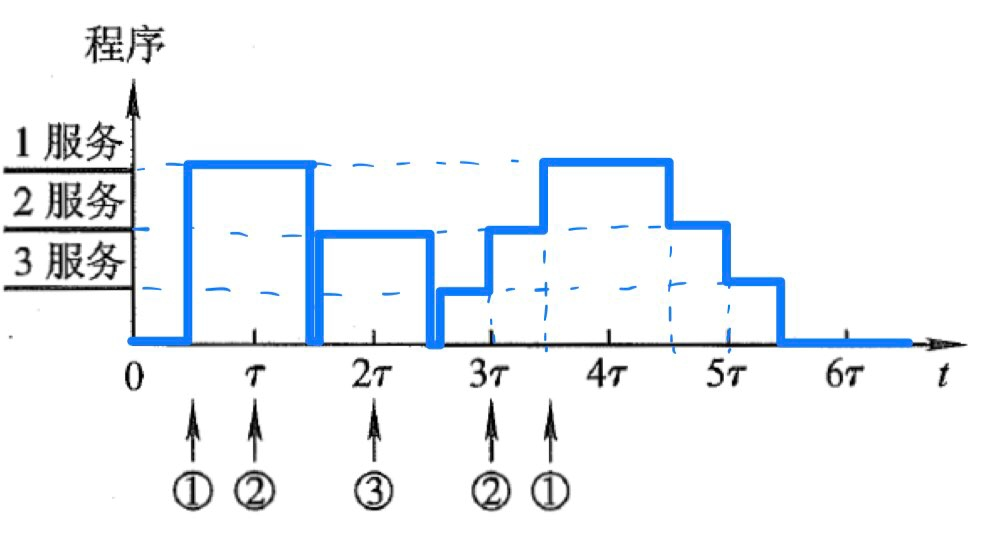
\includegraphics[width=8cm]{fig/8.27.png}
        \caption{题8.27}
        \label{fig:8_27}
    \end{figure}
\end{solution}
    

\problem{8.28} 设某机有$4$个中断源$1,\ 2,\ 3,\ 4$, 其响应优先级按$1 \to 2 \to 3 \to 4$降序排列, 现要求将中断处理次序改为$4 \to 1 \to 3 \to 2$, 根据下图给出的$4$个中断源的请求时刻, 画出CPU执行程序的轨迹. 设每个中断源的中断服务程序时间均为$20 \mathop{}\!\mu \mrm s$.

\begin{solution}
    如图\ref{fig:8_28}所示. 
    \begin{figure}[htbp]
        \centering
        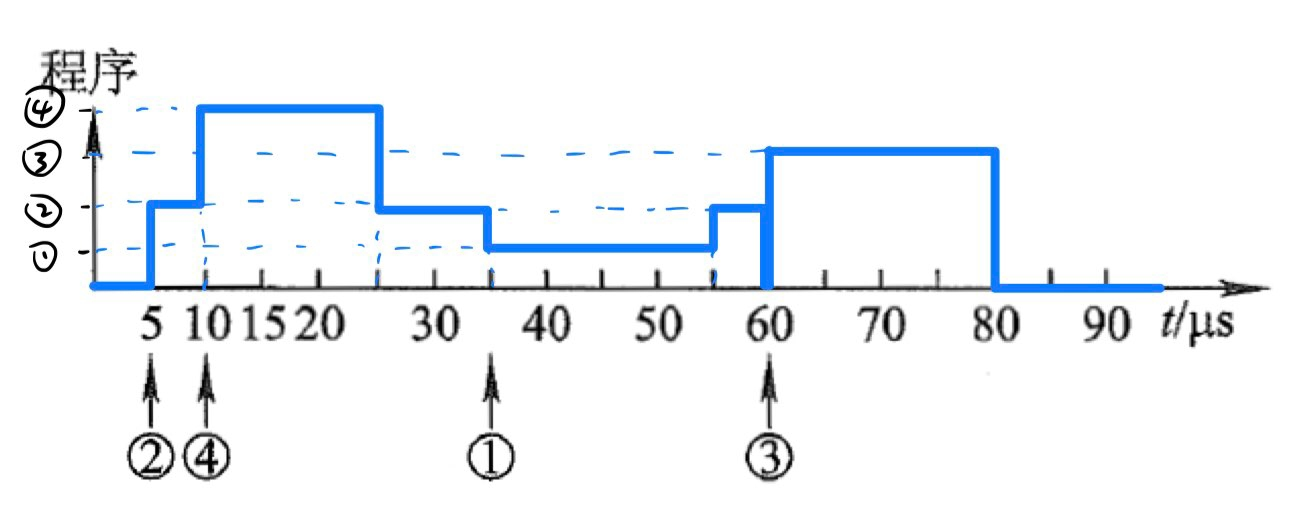
\includegraphics[width=8cm]{fig/8.28.png}
        \caption{题8.28}
        \label{fig:8_28}
    \end{figure}
\end{solution}
    












\end{document}